% Created by tikzDevice version 0.10.1 on 2020-02-15 16:16:49
% !TEX encoding = UTF-8 Unicode
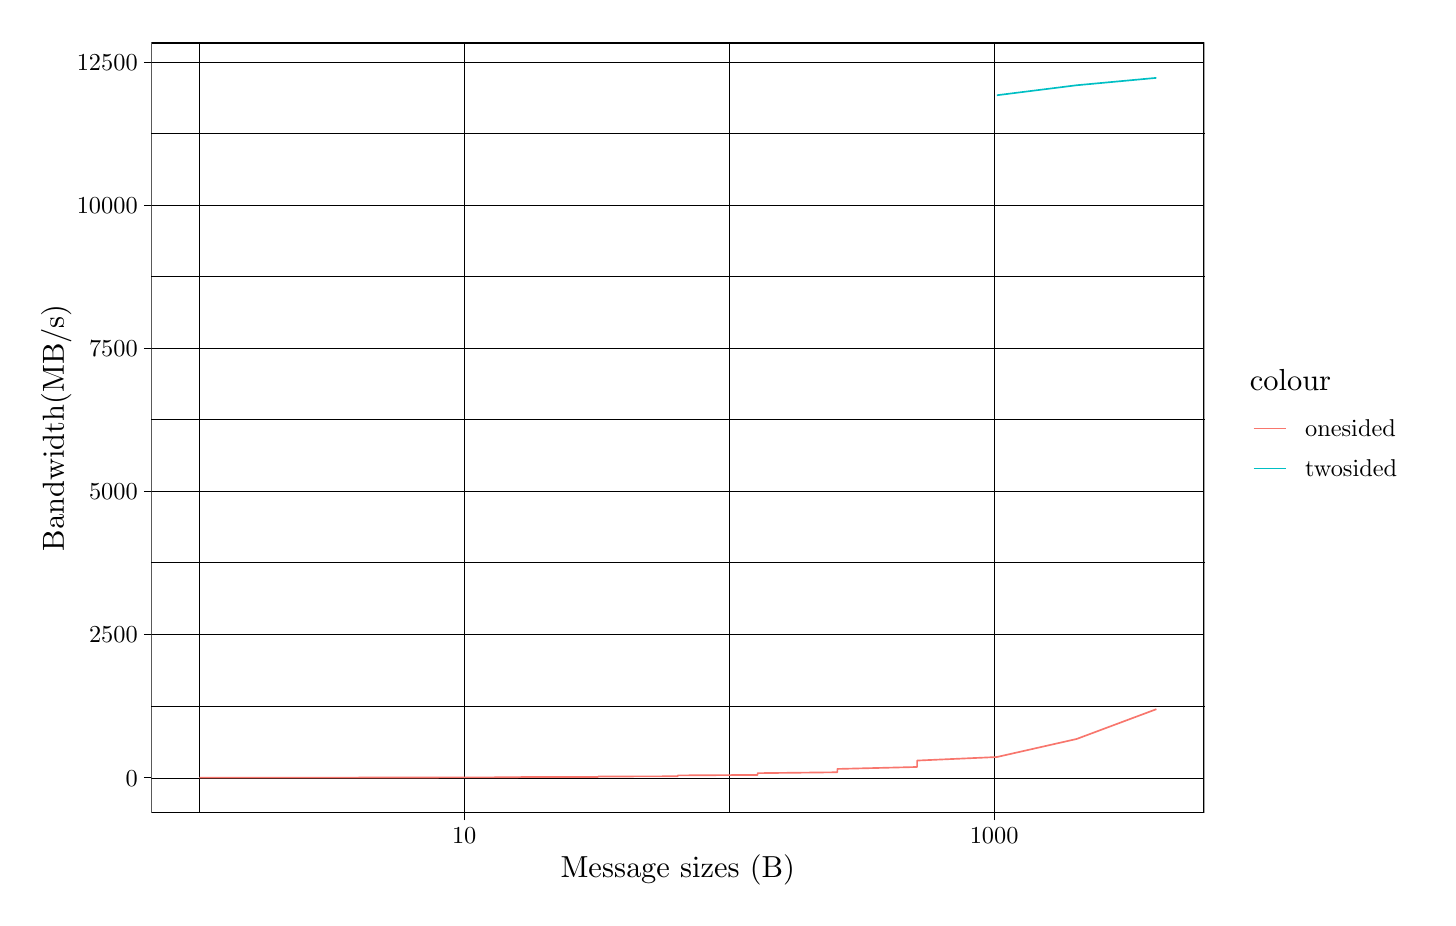
\begin{tikzpicture}[x=1pt,y=1pt]
\definecolor{fillColor}{RGB}{255,255,255}
\path[use as bounding box,fill=fillColor,fill opacity=0.00] (0,0) rectangle (505.89,314.37);
\begin{scope}
\path[clip] (  0.00,  0.00) rectangle (505.89,314.37);
\definecolor{drawColor}{RGB}{255,255,255}
\definecolor{fillColor}{RGB}{255,255,255}

\path[draw=drawColor,line width= 0.6pt,line join=round,line cap=round,fill=fillColor] (  0.00,  0.00) rectangle (505.89,314.37);
\end{scope}
\begin{scope}
\path[clip] ( 44.71, 30.72) rectangle (425.15,308.87);
\definecolor{fillColor}{RGB}{255,255,255}

\path[fill=fillColor] ( 44.71, 30.72) rectangle (425.15,308.87);
\definecolor{drawColor}{RGB}{0,0,0}

\path[draw=drawColor,line width= 0.0pt,line join=round] ( 44.71, 69.22) --
	(425.15, 69.22);

\path[draw=drawColor,line width= 0.0pt,line join=round] ( 44.71,120.93) --
	(425.15,120.93);

\path[draw=drawColor,line width= 0.0pt,line join=round] ( 44.71,172.64) --
	(425.15,172.64);

\path[draw=drawColor,line width= 0.0pt,line join=round] ( 44.71,224.35) --
	(425.15,224.35);

\path[draw=drawColor,line width= 0.0pt,line join=round] ( 44.71,276.07) --
	(425.15,276.07);

\path[draw=drawColor,line width= 0.0pt,line join=round] ( 62.01, 30.72) --
	( 62.01,308.87);

\path[draw=drawColor,line width= 0.0pt,line join=round] (253.49, 30.72) --
	(253.49,308.87);

\path[draw=drawColor,line width= 0.1pt,line join=round] ( 44.71, 43.36) --
	(425.15, 43.36);

\path[draw=drawColor,line width= 0.1pt,line join=round] ( 44.71, 95.07) --
	(425.15, 95.07);

\path[draw=drawColor,line width= 0.1pt,line join=round] ( 44.71,146.79) --
	(425.15,146.79);

\path[draw=drawColor,line width= 0.1pt,line join=round] ( 44.71,198.50) --
	(425.15,198.50);

\path[draw=drawColor,line width= 0.1pt,line join=round] ( 44.71,250.21) --
	(425.15,250.21);

\path[draw=drawColor,line width= 0.1pt,line join=round] ( 44.71,301.92) --
	(425.15,301.92);

\path[draw=drawColor,line width= 0.1pt,line join=round] (157.75, 30.72) --
	(157.75,308.87);

\path[draw=drawColor,line width= 0.1pt,line join=round] (349.23, 30.72) --
	(349.23,308.87);
\definecolor{drawColor}{RGB}{248,118,109}

\path[draw=drawColor,line width= 0.6pt,line join=round] ( 62.01, 43.37) --
	( 62.01, 43.37) --
	( 90.83, 43.38) --
	( 90.83, 43.39) --
	(119.65, 43.39) --
	(119.65, 43.41) --
	(148.47, 43.42) --
	(148.47, 43.46) --
	(177.29, 43.49) --
	(177.29, 43.57) --
	(206.11, 43.61) --
	(206.11, 43.77) --
	(234.93, 43.86) --
	(234.93, 44.18) --
	(263.75, 44.35) --
	(263.75, 44.99) --
	(292.57, 45.31) --
	(292.57, 46.51) --
	(321.40, 47.22) --
	(321.40, 49.54) --
	(350.22, 50.82) --
	(379.04, 57.34) --
	(407.86, 68.11);
\definecolor{drawColor}{RGB}{0,191,196}

\path[draw=drawColor,line width= 0.6pt,line join=round] (350.22,289.95) --
	(379.04,293.56) --
	(407.86,296.23);
\definecolor{drawColor}{RGB}{0,0,0}

\path[draw=drawColor,line width= 0.6pt,line join=round,line cap=round] ( 44.71, 30.72) rectangle (425.15,308.87);
\end{scope}
\begin{scope}
\path[clip] (  0.00,  0.00) rectangle (505.89,314.37);
\definecolor{drawColor}{RGB}{0,0,0}

\node[text=drawColor,anchor=base east,inner sep=0pt, outer sep=0pt, scale=  0.88] at ( 39.76, 40.33) {0};

\node[text=drawColor,anchor=base east,inner sep=0pt, outer sep=0pt, scale=  0.88] at ( 39.76, 92.04) {2500};

\node[text=drawColor,anchor=base east,inner sep=0pt, outer sep=0pt, scale=  0.88] at ( 39.76,143.75) {5000};

\node[text=drawColor,anchor=base east,inner sep=0pt, outer sep=0pt, scale=  0.88] at ( 39.76,195.47) {7500};

\node[text=drawColor,anchor=base east,inner sep=0pt, outer sep=0pt, scale=  0.88] at ( 39.76,247.18) {10000};

\node[text=drawColor,anchor=base east,inner sep=0pt, outer sep=0pt, scale=  0.88] at ( 39.76,298.89) {12500};
\end{scope}
\begin{scope}
\path[clip] (  0.00,  0.00) rectangle (505.89,314.37);
\definecolor{drawColor}{RGB}{0,0,0}

\path[draw=drawColor,line width= 0.3pt,line join=round] ( 41.96, 43.36) --
	( 44.71, 43.36);

\path[draw=drawColor,line width= 0.3pt,line join=round] ( 41.96, 95.07) --
	( 44.71, 95.07);

\path[draw=drawColor,line width= 0.3pt,line join=round] ( 41.96,146.79) --
	( 44.71,146.79);

\path[draw=drawColor,line width= 0.3pt,line join=round] ( 41.96,198.50) --
	( 44.71,198.50);

\path[draw=drawColor,line width= 0.3pt,line join=round] ( 41.96,250.21) --
	( 44.71,250.21);

\path[draw=drawColor,line width= 0.3pt,line join=round] ( 41.96,301.92) --
	( 44.71,301.92);
\end{scope}
\begin{scope}
\path[clip] (  0.00,  0.00) rectangle (505.89,314.37);
\definecolor{drawColor}{RGB}{0,0,0}

\path[draw=drawColor,line width= 0.3pt,line join=round] (157.75, 27.97) --
	(157.75, 30.72);

\path[draw=drawColor,line width= 0.3pt,line join=round] (349.23, 27.97) --
	(349.23, 30.72);
\end{scope}
\begin{scope}
\path[clip] (  0.00,  0.00) rectangle (505.89,314.37);
\definecolor{drawColor}{RGB}{0,0,0}

\node[text=drawColor,anchor=base,inner sep=0pt, outer sep=0pt, scale=  0.88] at (157.75, 19.71) {10};

\node[text=drawColor,anchor=base,inner sep=0pt, outer sep=0pt, scale=  0.88] at (349.23, 19.71) {1000};
\end{scope}
\begin{scope}
\path[clip] (  0.00,  0.00) rectangle (505.89,314.37);
\definecolor{drawColor}{RGB}{0,0,0}

\node[text=drawColor,anchor=base,inner sep=0pt, outer sep=0pt, scale=  1.10] at (234.93,  7.44) {Message sizes (B)};
\end{scope}
\begin{scope}
\path[clip] (  0.00,  0.00) rectangle (505.89,314.37);
\definecolor{drawColor}{RGB}{0,0,0}

\node[text=drawColor,rotate= 90.00,anchor=base,inner sep=0pt, outer sep=0pt, scale=  1.10] at ( 13.08,169.80) {Bandwidth(MB/s)};
\end{scope}
\begin{scope}
\path[clip] (  0.00,  0.00) rectangle (505.89,314.37);
\definecolor{fillColor}{RGB}{255,255,255}

\path[fill=fillColor] (436.15,142.34) rectangle (500.39,197.26);
\end{scope}
\begin{scope}
\path[clip] (  0.00,  0.00) rectangle (505.89,314.37);
\definecolor{drawColor}{RGB}{0,0,0}

\node[text=drawColor,anchor=base west,inner sep=0pt, outer sep=0pt, scale=  1.10] at (441.65,183.22) {colour};
\end{scope}
\begin{scope}
\path[clip] (  0.00,  0.00) rectangle (505.89,314.37);
\definecolor{fillColor}{RGB}{255,255,255}

\path[fill=fillColor] (441.65,162.29) rectangle (456.10,176.74);
\end{scope}
\begin{scope}
\path[clip] (  0.00,  0.00) rectangle (505.89,314.37);
\definecolor{drawColor}{RGB}{248,118,109}

\path[draw=drawColor,line width= 0.6pt,line join=round] (443.10,169.52) -- (454.66,169.52);
\end{scope}
\begin{scope}
\path[clip] (  0.00,  0.00) rectangle (505.89,314.37);
\definecolor{drawColor}{RGB}{248,118,109}

\path[draw=drawColor,line width= 0.6pt,line join=round] (443.10,169.52) -- (454.66,169.52);
\end{scope}
\begin{scope}
\path[clip] (  0.00,  0.00) rectangle (505.89,314.37);
\definecolor{fillColor}{RGB}{255,255,255}

\path[fill=fillColor] (441.65,147.84) rectangle (456.10,162.29);
\end{scope}
\begin{scope}
\path[clip] (  0.00,  0.00) rectangle (505.89,314.37);
\definecolor{drawColor}{RGB}{0,191,196}

\path[draw=drawColor,line width= 0.6pt,line join=round] (443.10,155.06) -- (454.66,155.06);
\end{scope}
\begin{scope}
\path[clip] (  0.00,  0.00) rectangle (505.89,314.37);
\definecolor{drawColor}{RGB}{0,191,196}

\path[draw=drawColor,line width= 0.6pt,line join=round] (443.10,155.06) -- (454.66,155.06);
\end{scope}
\begin{scope}
\path[clip] (  0.00,  0.00) rectangle (505.89,314.37);
\definecolor{drawColor}{RGB}{0,0,0}

\node[text=drawColor,anchor=base west,inner sep=0pt, outer sep=0pt, scale=  0.88] at (461.60,166.49) {onesided};
\end{scope}
\begin{scope}
\path[clip] (  0.00,  0.00) rectangle (505.89,314.37);
\definecolor{drawColor}{RGB}{0,0,0}

\node[text=drawColor,anchor=base west,inner sep=0pt, outer sep=0pt, scale=  0.88] at (461.60,152.03) {twosided};
\end{scope}
\end{tikzpicture}
